%%==================================================================%%
%% Author : Sa�udo Olmedo, Ignacio                                  %%
%% Author : S�nchez Barreiro, Pablo                                 %%
%% Version: 1.5, 15/05/2014                                         %%
%%                                                                  %%
%% Memoria del Proyecto Fin de Carrera                              %%
%% m2t/Caso de estudio                                              %%
%%==================================================================%%

Una vez definido el funcionamiento del generador de c�digo podemos continuar con el caso de estudio planteado en el segundo cap�tulo sobre Twissandra. Como se present� anteriormente el objetivo de este caso de estudio es la generaci�n de c�digo CQL a partir de un modelo UML 2.0. Para ello definimos una serie de reglas de transformaci�n entre modelos y obtuvimos un modelo de Cassandra a partir de un modelo UML que representaba una versi�n simplificada de Twitter llamada Twissandra.
En esta secci�n se presenta el resultado de la transformaci�n del modelo de Twissandra a c�digo.

Tras obtener el modelo Cassandra de Twissandra (figura~\ref{back:fig:modeloTwissandra}) y tras la definici�n del generador de c�digo se pone en funcionamiento la transformaci�n modelo-c�digo. El resultado de la transformaci�n se detalla a continuaci�n.El c�digo resultante tras ejecutar el generador de c�digo es el siguiente (figura~\ref{back:code:codigoCass}).

\begin{figure}[!tb]
  \centering
  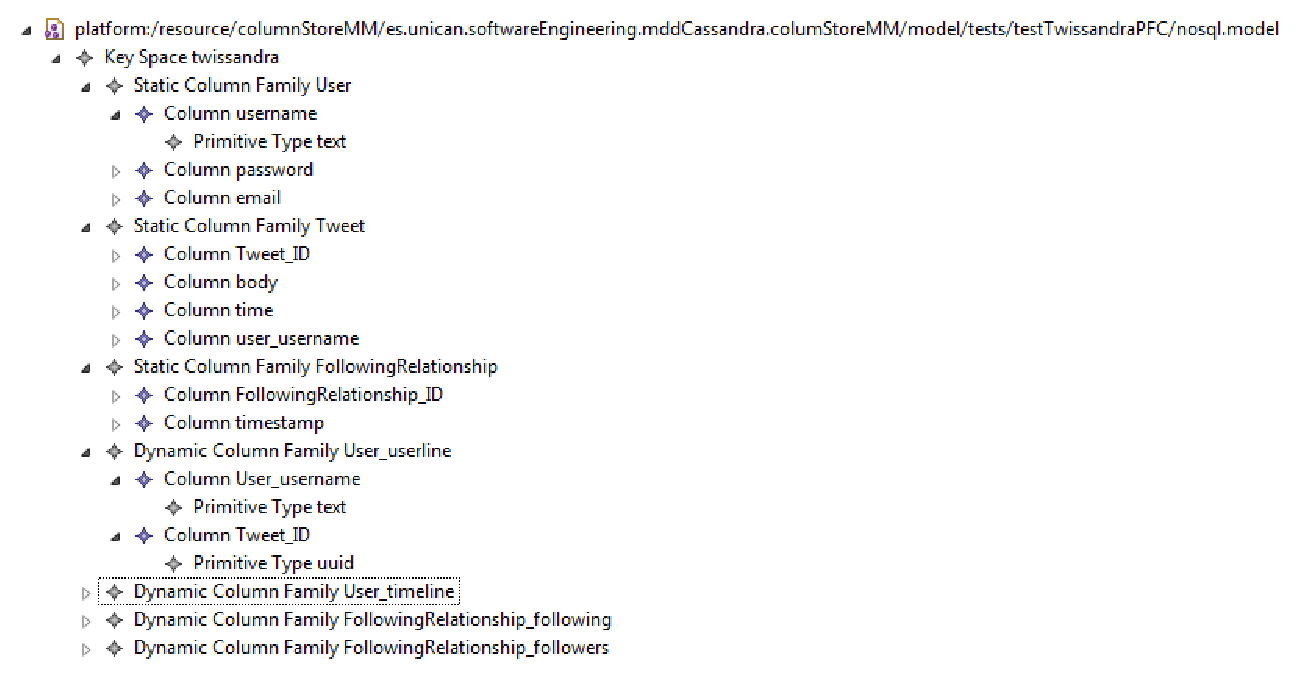
\includegraphics[width=.8\linewidth]{m2t/images/modeloTwissandra.eps} \\
  \caption{Modelo UML Twissandra}
  \label{back:fig:modeloTwissandra}
\end{figure}

Como vemos en el c�digo las tres primeras l�neas son para borrar el keyspace en caso de que existiera, crearlo y configurar la arquitectura de replicaci�n seg�n estaba especificado en el modelo Cassandra. A continuaci�n se conecta la sesi�n con el keyspace correspondiente.
Por cada column family (sea est�tica o din�mica) se genera un bloque \"CREATE TABLE\". Cada columna de la column family es transformada en una columna de la tabla. La transformaci�n como se contaba en la secci�n anterior es trivial, sin embargo el problema del generador de c�digo surge a la hora de definir la estructura de la primary key. Las column family est�ticas siguen una definici�n de claves tradicional, sin embargo las column families din�micas tienen que tener en cuenta que las claves de partici�n (partition keys) pueden ser compuestas (aunque en este ejemplo no existen). Por ejemplo el caso de user\_userline las columnas user\_name y tweet\_id son designadas como primary key, user\_username ser� la clave de partici�n.


\begin{figure}[!tb]
\begin{center}
\begin{footnotesize}
\begin{verbatim}
DROP KEYSPACE twissandra;
CREATE KEYSPACE twissandra
WITH replication = {'class':'SimpleStrategy', 'replication_factor':1};

USE twissandra;

CREATE TABLE User(
       username text,
       password text,
       email set<text>,
       PRIMARY KEY(username)
);

CREATE TABLE Tweet(
       Tweet_ID uuid,
       body text,
       time timestamp,
       user_username text,
       PRIMARY KEY(Tweet_ID)
);

CREATE TABLE FollowingRelationship(
       FollowingRelationship_ID uuid,
       timestamp timestamp,
       PRIMARY KEY(FollowingRelationship_ID)
);

CREATE TABLE User_userline(
       User_username text,
       Tweet_ID uuid,
       PRIMARY KEY((User_username),Tweet_ID)
);

CREATE TABLE User_timeline(
       User_username text,
       Tweet_ID uuid,
       PRIMARY KEY((User_username),Tweet_ID)
);

CREATE TABLE FollowingRelationship_following(
       FollowingRelationship_FollowingRelationship_ID uuid,
       username text,
       PRIMARY KEY((FollowingRelationship_FollowingRelationship_ID),username)
);

CREATE TABLE FollowingRelationship_followers(
       FollowingRelationship_FollowingRelationship_ID uuid,
       username text,
       PRIMARY KEY((FollowingRelationship_FollowingRelationship_ID),username)
);

\end{verbatim}
\end{footnotesize}
\end{center}
\caption{C�digo resultante Twissandra}
\label{back:code:codigoCass}
\end{figure}

